\chapter{Motivation und
Anforderungen}\label{motivation-und-anforderungen}

Kapitel~\ref{einleitung} hat Problemstellung und Zielsetzung des Systems eingeführt. Dieses Kapitel leitet daraus formale Anforderungen ab. Es analysiert die drei Anforderungsdimensionen redaktioneller Aufwand (Abschnitt~\ref{redaktioneller-aufwand-bei-livetickern}), Mehrsprachigkeit (Abschnitt~\ref{mehrsprachigkeit-als-herausforderung}) und White-Label-Bedarf (Abschnitt~\ref{white-label-bedarf-im-profisport}), konkretisiert diese am Fallbeispiel Eintracht Frankfurt (Abschnitt~\ref{anforderungsanalyse-am-beispiel-eintracht-frankfurt}) und fasst alle Anforderungen in einem formalen Pflichtenheft zusammen (Abschnitt~\ref{zusammenfassung-der-systemanforderungen}).

\section{Redaktioneller Aufwand bei
Livetickern}\label{redaktioneller-aufwand-bei-livetickern}


In Abständen von einer bis drei Minuten sind unter simultaner Beobachtung des Spielgeschehens Ereignisse wahrzunehmen, journalistisch zu bewerten, zu kontextualisieren und in sprachlich angemessene Form zu bringen (vgl. Hauser 2008, S.~3--4). Diese kognitive Parallelverarbeitung macht den Liveticker zu einer Echtzeit-Textgattung, die sich fundamental von retrospektiven Formaten wie dem Spielbericht unterscheidet (vgl. Hauser 2008, S.~2--3). Zusätzlich muss ein Ticker ein heterogenes Publikum gleichzeitig bedienen, da First-Screen-Nutzer ohne TV-Bild eine primäre Beschreibung des Spielgeschehens erwarten, während Second-Screen-Nutzer mit TV-Bild auf zusätzliche Einordnung und Unterhaltung angewiesen sind (vgl. McEnnis 2016, zit. n. Bluhm \& Schäfer 2023, S.~24 u.~36). Diese Doppelfunktion verschärft den Anforderungsdruck weiter, da der Text gleichzeitig faktisch korrekt, sprachlich angemessen und unterhaltsam sein muss (vgl. Meier 2018, zit. n. Bluhm \& Schäfer 2023, S.~27).

Verfassen und Redigieren fallen in einem einzigen Schritt zusammen (Walter 2020, S.~29). Zusätzlich müssen Ticker-Autoren häufig parallel weitere Aufgaben übernehmen, wie etwa die Erstellung des abschließenden Spielberichts (Bluhm \& Schäfer 2023, S.~35). Die Fehleranfälligkeit unter diesen Bedingungen ist systemimmanent. Zahlendreher bei Spielminuten, falsch zugeordnete Spielernamen oder stilistische Brüche innerhalb eines Tickers sind keine Ausnahme, sondern eine vorhersehbare Konsequenz des Produktionsdrucks (vgl. Walter 2020, S.~29; Bluhm \& Schäfer 2023, S.~35).

Das Skalierungsproblem verschärft sich an Spieltagen mit Parallelspielen erheblich. An einem typischen Bundesliga-Samstag finden bis zu sechs Partien zeitgleich statt (vgl. DFL 2024). Redaktionen, die für mehrere Spiele Ticker anbieten, müssen entweder entsprechend viele Autoren gleichzeitig einsetzen oder einzelne Autoren mehrere Ticker parallel betreuen lassen, mit absehbaren Qualitätseinbußen (vgl. Bluhm \& Schäfer 2023, S.~32, 35). Erschwerend kommt hinzu, dass Liveticker-Stellen häufig mit wechselndem freien Personal besetzt werden (Bluhm \& Schäfer 2023, S.~32) — konsistente Tonalität und sprachliches Niveau sind unter diesen Bedingungen manuell nicht zuverlässig zu gewährleisten. Für Vereinsredaktionen mit kleinen Teams ist eine rein manuelle Skalierung damit personell und wirtschaftlich kaum darstellbar. Dass diese strukturellen Grenzen selbst bei professionell aufgestellten Vereinsredaktionen spürbar werden, zeigt Abschnitt~\ref{anforderungsanalyse-am-beispiel-eintracht-frankfurt}.




\section{Mehrsprachigkeit als
Herausforderung}\label{mehrsprachigkeit-als-herausforderung}

Die Globalisierung des Profifußballs hat die Erwartungen an die Reichweite digitaler Inhalte grundlegend verändert. Internationale Fangemeinschaften erwarten heute eine mediale Begleitung in ihrer Landessprache. Am Beispiel der Premier League lässt sich dieser Wandel besonders deutlich illustrieren, da der internationale Markt für die Liga längst bedeutender ist als der heimische englische (vgl. Bertling, zit. n. Beils 2023, S.~221). Dies betrifft zunehmend auch Bundesliga-Vereine mit zweistelligen Millionen-Reichweiten auf globalen Plattformen (vgl. Beils 2023, S.~200). Eine rein deutschsprachige Berichterstattung wird dieser Reichweite nicht mehr gerecht. Für Bundesliga-Vereine ist Englisch die primäre Zielsprache, wie Abschnitt~\ref{fallstudie-eintracht-frankfurt} am Fallbeispiel Eintracht Frankfurt belegt.

Mehrsprachige Berichterstattung beschränkt sich nicht auf eine reine Übersetzung existierender Inhalte. Im Kontext von Sport-Livetickern variieren sprachliche Konventionen, idiomatische Wendungen und die emotionale Tonalität kulturspezifisch. Es handelt sich daher weniger um ein Übersetzungs- als um ein Lokalisierungsproblem. Jede weitere Sprache erfordert spezialisiertes Personal für Übersetzungs- und Anpassungsprozesse, was unter den ohnehin ressourcenknappen Echtzeit-Bedingungen die wirtschaftlichen und personellen Kapazitäten der meisten Vereinsredaktionen übersteigt (vgl. Bluhm \& Schäfer 2023, S.~32). Die Mehrsprachigkeit stellt damit eine eigenständige Systemanforderung dar, die über redaktionelle Kapazitätsgrenzen hinaus technologische Unterstützung erfordert.




\section{White-Label-Bedarf im
Profisport}\label{white-label-bedarf-im-profisport}

Vereine kommunizieren heute zunehmend direkt mit ihrer Anhängerschaft und haben eigene Redaktionen aufgebaut (vgl. Beils 2023, S.~155). Anders als überregionale Medien betrachten Vereinsticker die Partie aus der Perspektive der eigenen Fans (vgl. Canalp, zit. n. Beils 2023, S.~57), weshalb Ereignisse je nach Kanal unterschiedlich getönt sein müssen. Der Vereinskanal spricht emotionale Fanbindung an, während neutrale Plattformen sachliche Information priorisieren. Bei anhaltenden Rückständen oder schwachen Leistungen des eigenen Teams kann darüber hinaus ein kritisch-analysierender Stil angemessener sein als unkritische Euphorie. Da jeder Verein einen eigenen Kommunikationsstil pflegt, ist die stilistische Ausprägung vereinsindividuell und lässt sich nicht auf eine universelle Vorlage reduzieren.

Diese Variabilität konsistent einzuhalten stellt Redaktionen vor eine eigenständige Herausforderung. Die in Abschnitt~\ref{redaktioneller-aufwand-bei-livetickern} beschriebene personelle Fluktuation verschärft dies zusätzlich. Die Markenstimme muss systemseitig konfigurierbar sein.

Dieses Konsistenzproblem lässt sich durch \textbf{White-Label-Architekturen} technisch adressieren (vgl. Pohl et al.\ 2005, S.~12). Ein generisches Kernsystem wird so konzipiert, dass es für verschiedene Abnehmer individuell konfigurierbar ist, ohne den Quellcode zu ändern. Auf die Liveticker-Produktion übertragen bedeutet dies, dass eine einzige Codebasis für beliebige Vereine instanziierbar sein muss, ohne dass für jeden Verein eine separate Implementierung gepflegt wird. Datenquellen, Medieneinbindungen und Stilkonfiguration müssen dabei vollständig über Parameter steuerbar sein.

Der folgende Abschnitt konkretisiert diese Anforderungen am Fallbeispiel Eintracht Frankfurt.



\section{Fallstudie Eintracht
Frankfurt}\label{anforderungsanalyse-am-beispiel-eintracht-frankfurt}

Grundlage ist ein leitfadengestütztes Experteninterview mit dem Digitalverantwortlichen des Vereins, ergänzt durch Beobachtungen im Projektzeitraum.

\subsection{Vereinsspezifische Betriebskennzahlen}\label{fallstudie-eintracht-frankfurt}

Eintracht Frankfurt bestreitet pro Saison bis zu 60 Pflichtspiele. Pro Spiel fallen typischerweise 60--120 Ticker-Einträge an, wobei die genaue Zahl von der Ereignisdichte abhängt (vgl.\ Abschnitt~\ref{experteninterview-leitfaden}). Die Liveticker-Produktion übernimmt ein zweiköpfiges Team aus Redakteur und technischem Administrator. Das Team arbeitet stets vor Ort im Stadion, auch bei Auswärtsspielen. Der Redakteur fokussiert sich dabei ausschließlich auf Ticker-Inhalte einschließlich Bildauswahl und Medieneinbettung. Als explizites Geschwindigkeitsziel gilt, früher als konkurrierende Medien wie Kicker oder Bundesliga.de zu publizieren (vgl.\ Abschnitt~\ref{experteninterview-leitfaden}). Als ergänzende Zielsprache wurde im Interview Englisch als relevant für die internationale Fanbasis des Vereins bestätigt.

Der vereinsspezifische Ticker-Stil ist emotional und parteiisch zugunsten Eintrachts, jedoch nicht unsachlich. Er ist fan-nah, mit klarer Eintracht-Sprache und typisch hessischer Färbung (vgl.\ Abschnitt~\ref{experteninterview-leitfaden}). Klare Stilrichtlinien für den Eintracht-Ton sind vorhanden; das bestehende System kann sie weder einfordern noch vorschlagen.



\subsection{Ist-Zustand: Bestehendes Redaktionssystem}\label{ist-zustand-bestehendes-system}

Als Ausgangspunkt illustriert Abbildung~\ref{fig:altsystem} den konkreten Ist-Zustand anhand des im Projektzeitraum eingesetzten Redaktionssystems bei Eintracht Frankfurt. Es handelt sich um ein eigens entwickeltes Backend des Website-Dienstleisters, über dessen Schnittstelle Ticker-Einträge in die vereinseigene App ausgespielt werden. Das System repräsentiert den Stand eines rein manuellen Werkzeugs ohne KI-Integration.

\begin{figure}[H]
\centering
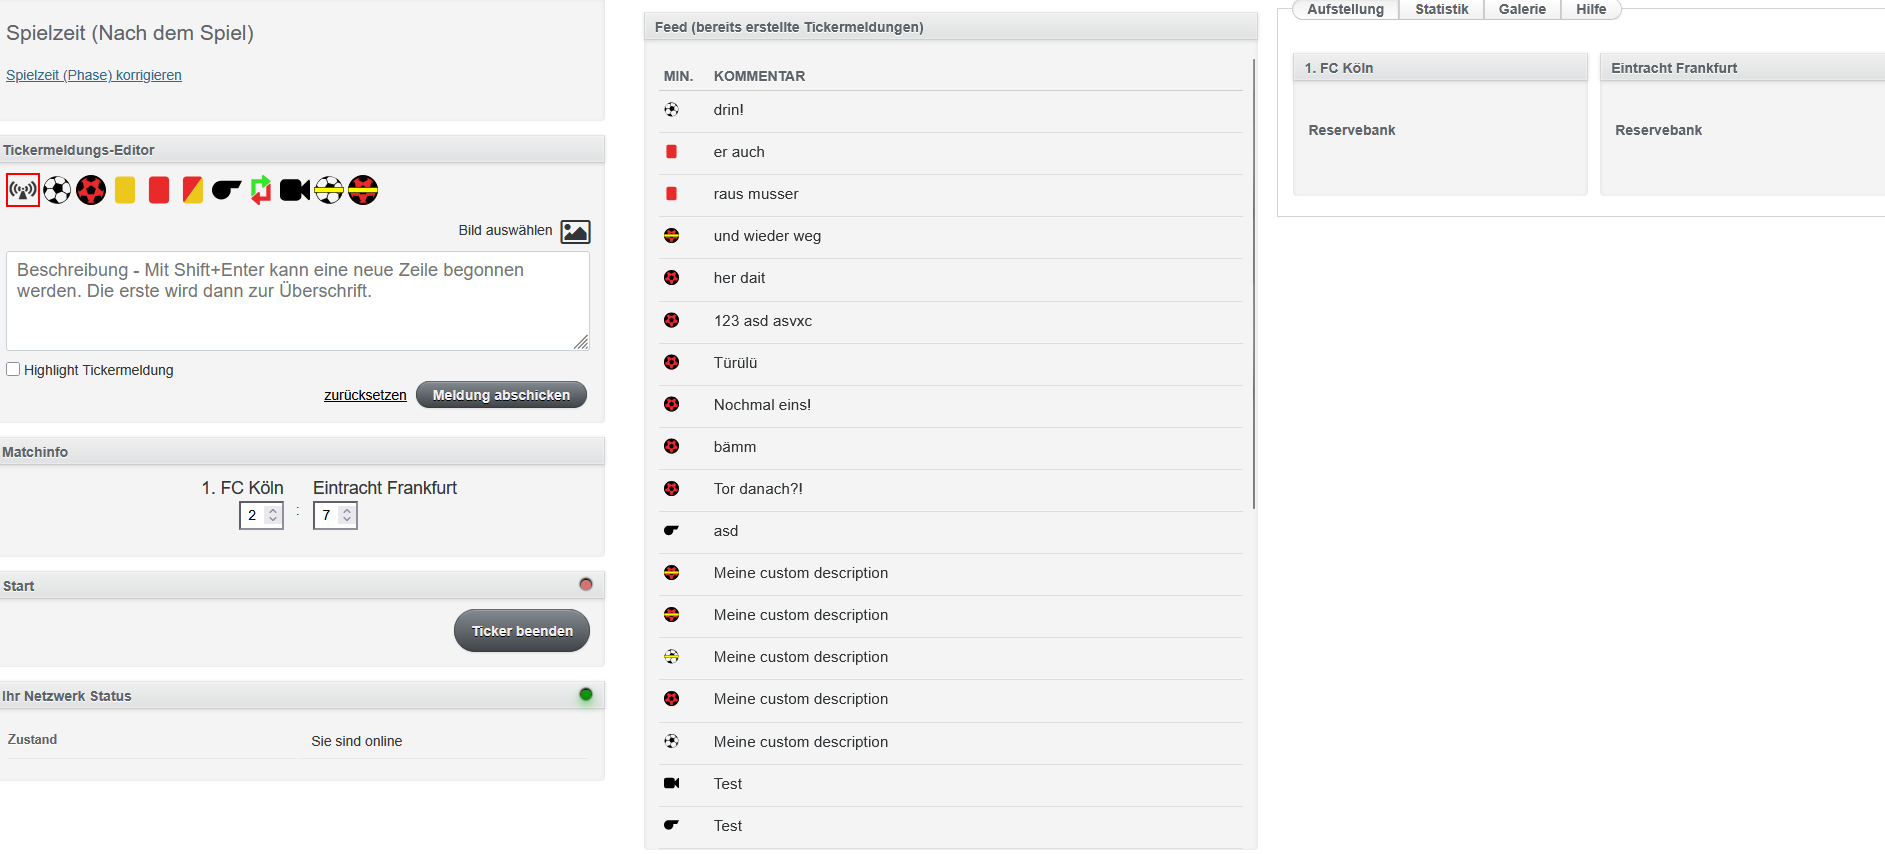
\includegraphics[width=0.95\textwidth]{altsystem_eintracht.png}
\caption[Bestehendes Liveticker-Redaktionssystem (Eintracht Frankfurt, Saison 2024/25)]{Bestehendes Liveticker-Redaktionssystem bei Eintracht Frankfurt (Stand: Saison 2024/25). Links: Ticker-Editor mit manueller Score-Pflege. Mitte: Feed bereits erstellter Meldungen. Rechts: Aufstellungs-Panel im Leerzustand ohne geladene Spielerdaten.}
\label{fig:altsystem}
\end{figure}

Die Systemanalyse zeigt sechs strukturelle Defizite, die den Handlungsbedarf für das in dieser Arbeit entwickelte System begründen:

\begin{itemize}\tightlist
\item \textbf{Kein KI-Vorschlag und keine technische Stilunterstützung:} Der Ticker-Editor ist ein reines Freitextfeld ohne KI-Unterstützung oder Vorschlagsfunktion. Obwohl klare redaktionelle Richtlinien für den Eintracht-Stil vorhanden sind, kann das System diese weder einfordern noch vorschlagen (vgl.\ Abschnitt~\ref{experteninterview-leitfaden}).
\item \textbf{Manuelle Score-Pflege:} Der Spielstand wird über numerische Eingabefelder manuell gepflegt (Abbildung~\ref{fig:altsystem}, links unten). Obwohl der Verein externe Datenquellen (Opta, DFBnet) für Livedaten nutzt, ist keine automatische Synchronisation dieser Feeds mit der Liveticker-Oberfläche vorhanden. Die Daten sind grundsätzlich zuverlässig, jedoch anfällig für Verzögerungen und Fehlzuordnungen, etwa bei kurzfristigen Aufstellungsänderungen oder instabiler Internetverbindung im Auswärtsstadion, weshalb manuelle Korrekturen durch Redakteure essenziell bleiben (vgl.\ Abschnitt~\ref{experteninterview-leitfaden}).
\item \textbf{Keine Medienintegration:} Das System bietet lediglich einen einfachen „Bild auswählen''-Button ohne strukturierte Social-Media-Anbindung, Galeriefunktion oder automatischen Medien-Import (z.\,B. ScorePlay, YouTube, Instagram).
\item \textbf{Fehlender Mehrsprachen-Support:} Das System ist ausschließlich deutschsprachig ausgelegt. Eine Übersetzungsfunktion oder mehrsprachige Textgenerierung ist nicht vorgesehen.
\item \textbf{Fehlende Live-Statistiken und Medieneinbettung:} Aufstellungsdaten werden laut Experteninterview bereits automatisiert übertragen; eine Integration von Live-Statistiken sowie audiovisuellen Inhalten fehlt jedoch vollständig. Im Interview wurde bestätigt: „Videos und Audios können wir noch nicht darstellen, Statistiken ebenso'' (vgl.\ Abschnitt~\ref{experteninterview-leitfaden}).
\item \textbf{Systemkomplexität und Fehleranfälligkeit:} Das Backend besteht aus zahlreichen Sonderlösungen und ist entsprechend komplex. Für Redakteure, die das System nicht gut kennen, erhöht dies die Fehleranfälligkeit im laufenden Betrieb erheblich (vgl.\ Abschnitt~\ref{experteninterview-leitfaden}).
\end{itemize}

Diese Defizite spiegeln die drei in Abschnitt~\ref{problemstellung-und-zielsetzung} identifizierten Anforderungsdimensionen direkt wider: operativer Zeitdruck durch vollständig manuelle Produktion, fehlende Mehrsprachigkeit und eingeschränkte White-Label-Fähigkeit. Wie Kapitel~\ref{systemkonzeption} und Abschnitt~\ref{anforderungsabgleich-soll-ist-vergleich} zeigen, adressiert das entwickelte System alle sechs Defizite.




\section{Zusammenfassung der
Systemanforderungen}\label{zusammenfassung-der-systemanforderungen}

Die folgenden 19 Anforderungen fassen die aus den Anforderungsdimensionen hergeleiteten Systemeigenschaften zusammen. Sie gliedern sich in funktionale Anforderungen (Abschnitt~\ref{funktionale-anforderungen}) und Qualitätsanforderungen (Abschnitt~\ref{nicht-funktionale-anforderungen}). Abschnitt~\ref{anforderungsabgleich-soll-ist-vergleich} gleicht jeden Punkt mit dem implementierten Stand ab.

\subsection{Funktionale Anforderungen}\label{funktionale-anforderungen}

{\def\LTcaptype{none} % do not increment counter
\begin{longtable}[]{@{}
  >{\raggedright\arraybackslash}p{(\linewidth - 4\tabcolsep) * \real{0.0370}}
  >{\raggedright\arraybackslash}p{(\linewidth - 4\tabcolsep) * \real{0.6667}}
  >{\raggedright\arraybackslash}p{(\linewidth - 4\tabcolsep) * \real{0.2963}}@{}}
\toprule\noalign{}
\begin{minipage}[b]{\linewidth}\raggedright
Nr.
\end{minipage} & \begin{minipage}[b]{\linewidth}\raggedright
Anforderung
\end{minipage} & \begin{minipage}[b]{\linewidth}\raggedright
Herleitung
\end{minipage} \\
\midrule\noalign{}
\endhead
\bottomrule\noalign{}
\endlastfoot
F1 & Drei Betriebsmodi (\texttt{auto}, \texttt{coop}, \texttt{manual}) & Kap.~\ref{problemstellung-und-zielsetzung}, \ref{redaktioneller-aufwand-bei-livetickern} \\
F2 & KI-Textgenerierung für alle Event-Typen & Kap.~\ref{redaktioneller-aufwand-bei-livetickern}, \ref{anforderungsanalyse-am-beispiel-eintracht-frankfurt} \\
F3 & Drei Stilprofile (neutral, euphorisch, kritisch) & Kap.~\ref{white-label-bedarf-im-profisport} \\
F4 & Stilkonfiguration über vereinsspezifische Referenztexte & Kap.~\ref{white-label-bedarf-im-profisport} \\
F5 & Ticker-Lifecycle (draft → published / rejected / deleted) & Kap.~\ref{redaktioneller-aufwand-bei-livetickern} \\
F6 & Schnelle manuelle Ticker-Erstellung im \texttt{manual}-Modus & Kap.~\ref{redaktioneller-aufwand-bei-livetickern} (Zeitdruck) \\
F7 & Mehrsprachige Textgenerierung (Deutsch, Englisch, Spanisch, Französisch) & Kap.~\ref{mehrsprachigkeit-als-herausforderung} \\
F8 & Automatischer, idempotenter ETL-Datenimport aus externen Sportdatenquellen & Kap.~\ref{redaktioneller-aufwand-bei-livetickern}, \ref{anforderungsanalyse-am-beispiel-eintracht-frankfurt} (Echtzeit-Betrieb) \\
F9 & Anbieterunabhängige LLM-Integration mit Ausfallsicherheit & Kap.~\ref{redaktioneller-aufwand-bei-livetickern} (Verfügbarkeit) \\
F10 & Deduplizierung von Ticker-Einträgen & Kap.~\ref{redaktioneller-aufwand-bei-livetickern} (Korrektheit) \\
F11 & Pre-Match-Kontextgenerierung (Verletzungen, H2H-Daten, Spielortinformationen) & Kap.~\ref{redaktioneller-aufwand-bei-livetickern} (Elaboration) \\
F12 & Live-Statistik-Updates & Kap.~\ref{redaktioneller-aufwand-bei-livetickern} (Echtzeit) \\
F13 & Medienintegration (ScorePlay-Bildmaterial, Social-Media-Panels für YouTube, X, Instagram) & Kap.~\ref{ist-zustand-bestehendes-system} (Defizit: fehlende Medienintegration im Altsystem) \\
F14 & Spielphasen-Management (Anpfiff, Halbzeit, Abpfiff) & Kap.~\ref{redaktioneller-aufwand-bei-livetickern} (Echtzeit-Betrieb) \\
F15 & Undo nach Publikation & Kap.~\ref{redaktioneller-aufwand-bei-livetickern} (Fehleranfälligkeit unter Zeitdruck) \\
F16 & REST-API zur vollständigen Systemsteuerung und Mandantenkonfiguration & Kap.~\ref{white-label-bedarf-im-profisport} (White-Label) \\
F17 & White-Label-Fähigkeit (vereinsspezifische und generische Instanz) & Kap.~\ref{white-label-bedarf-im-profisport}, \ref{anforderungsanalyse-am-beispiel-eintracht-frankfurt} \\
\end{longtable}
}

\subsection{Qualitätsanforderungen}\label{nicht-funktionale-anforderungen}

{\def\LTcaptype{none} % do not increment counter
\begin{longtable}[]{@{}
  >{\raggedright\arraybackslash}p{(\linewidth - 4\tabcolsep) * \real{0.0469}}
  >{\raggedright\arraybackslash}p{(\linewidth - 4\tabcolsep) * \real{0.5938}}
  >{\raggedright\arraybackslash}p{(\linewidth - 4\tabcolsep) * \real{0.3594}}@{}}
\toprule\noalign{}
\begin{minipage}[b]{\linewidth}\raggedright
Nr.
\end{minipage} & \begin{minipage}[b]{\linewidth}\raggedright
Anforderung
\end{minipage} & \begin{minipage}[b]{\linewidth}\raggedright
Herleitung
\end{minipage} \\
\midrule\noalign{}
\endhead
\bottomrule\noalign{}
\endlastfoot
N1 & Responsive UI (Mobile-tauglich) & Kap.~\ref{redaktioneller-aufwand-bei-livetickern} (Einsatzszenarien) \\
N2 & Fehlerresistenz im Frontend & Kap.~\ref{redaktioneller-aufwand-bei-livetickern} (Robustheit) \\
\end{longtable}
}


Die drei Anforderungsdimensionen (operativer Zeitdruck, Mehrsprachigkeit und White-Label-Bedarf) sind keine isolierten Herausforderungen, sondern greifen strukturell ineinander. Zeitdruck macht rein menschliche Skalierung kaum darstellbar, Mehrsprachigkeit multipliziert diesen Aufwand, und White-Label-Anforderungen verlangen eine stilistische Konsistenz, die wechselndes Personal nicht zuverlässig gewährleisten kann. Eine integrierte Lösung ist daher erforderlich. Die vorstehenden 19 Anforderungen bilden das Pflichtenheft für die Systemkonzeption in Kapitel~\ref{systemkonzeption}. Die hierfür notwendigen technologischen Grundlagen erschließt Kapitel~\ref{stand-der-technik}.
